\documentclass[UTF8]{article}
% \usepackage{ctex}
\usepackage{amsmath}
\usepackage{amssymb}
\usepackage{graphicx}
\usepackage{authblk}
\usepackage{natbib}
\usepackage{graphicx}
\usepackage{subfigure}
\usepackage{indentfirst}
\setlength{\parindent}{2em}

\begin{document}
\bibliographystyle{plain}
\author{Peisong Wen 1611450}
\title {Farewell vision part}
\date{}
\maketitle

\begin{abstract}
  We implemented farewell in kobuki chassis, which can help guests take coats, and send them to take cabs. In vision part, the first mission is to recognize and localize people who are waving their hands, and send the bounding boxes to navigation part. We use Openpose\cite{openpose} to  estimate human posture. The second mission is to detecte coats, and send the locations to robot arm part, help it catch the coat corresponding to the person who was waving hand. We use salience object detection with DRFI\cite{drfi}.
\newline

\textbf{Key words:farewell, human posture estimation, salience object detection}
\end{abstract}

\section{Introdution}
  \subsection{Main process}
    We have two main goals:help guests take their coats, and send them to take cabs. In the beginning, the robot is sleeping, waiting for orders. When it hears "I want to go", it will be wake up, looks around to find person who is waving hands, and records the specific ID by recognizing colors of his/her wearing. Then, it will go to where the coats are placed, with the camera focusing on the coats. It will detecte locations of all coats, find the coat corresponding to the recorded ID. After catching the coat, it will go back to the person, and give him/her the coat. The last step is leading he/she to where cabs are parked. That's all his jobs.
  \subsection{Vision part}
    We have two submission: detecte person waving his/her hand, and detecte coats.In the first mission, we have to detecte human pose keypoints. We choose Openpose, a human pose estimation model. It's fast, robust and insensitive to illumination, supported by a powerful dataset collected by CMU. We simply use the pretrained model. Then we judge where a person is waving with the spatial relations between head, elbow, wrist, and shoulder.

    In the second mission, what we need to do is object detection. To avoid collecting dataset, which is a quite tricky job, we use a unsupervise method called salience object detection to get a foreground confidence map, and cut object masks with a union-find set.

\section{Principle}
  \subsection{Pose estimation}
    Openpose is a open source human pose estimation model based on Caffe framework. It can detecte human keypoints like neck, elbow, wrist, shoulder and so on. It's fast botton-up method, which detecte keypoints firstly and then match keypoints belong to the same person.
    As Figure \ref{img_1} shows, input an RGB image, it will extract features by a convolution network. Then, it breaks into two branches, one extracts part confidence maps, the other one calculates part affinity fields(PAFs). Then it uses bipartite matching to get part association, builds a undirected graph describing the possibility that different keypoints belong to same person. At last, based on PAFs, it does multi-person parsing with ungarian algorithm.

    In fact we don't use all of the keypoints, so we can retrained the model to get better performance. However, we neither datasets nor powerful machines to train with, so we simply use the pretrained model.

    After extracting keypoints(head($P_h$), shoulder($P_s$), elbow($P_e$) and wrist($P_w$)), we use a naive method to judge whether a person is waving. Take the right side as an example, he/she is waving if keypoints meet the conditions:

    1.$P_w$ is above $\overrightarrow{P_hP_s}$, that is $\overrightarrow{P_hP_s} \times \overrightarrow{P_hP_w} > 0$

    2.$\angle P_sP_eP_w < \frac{\pi}{2}$

    \begin{figure}
      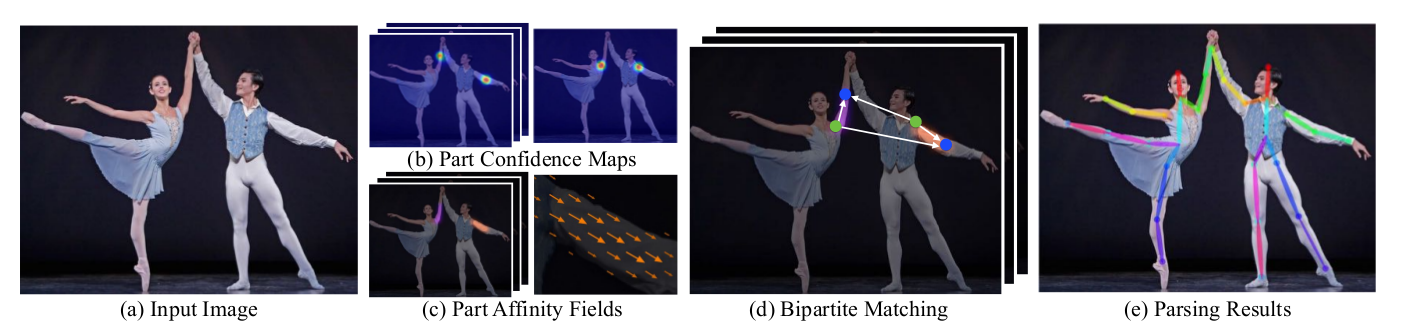
\includegraphics[width=\linewidth]{a.png}
      \caption{Openpose}
      \label{img_1}
      \end{figure}

  \subsection{Salience object detection}
    Since object detection is category related, we have to train a model with our own dataset if we use deep learning based methods like YOLO, SSD or faster-rcnn. To avoid such tricky work, we use a unsupervise method called salience object detection. Firstly, we calculate a salience confidence map for an input image with DRFI, a find out connected blocks with a union-find set after binarization.


\section{Experiment}
  In the vision part, the results are satisfactory. Openpose is excellent in both efficiency and accuracy, , as shown in Figure \ref{img_2}. Salience object detection has problems with messy background and occlusion, but if we placed the coats in a clear background and avoid occlusion, it can work well, as shown in .%Figure \ref{img_3}.
  However, human destiny is unpredictable, personal efforts are important but still depends on the history of history. We meet many problems when we combine our works. One of the common problems is that we are unable to connect to the master machine, for IP or ports errors. Another one problem is bandwidth limit, which causes blocking of some topics when we launch to many nodes. We have no idea T\_T.

  \begin{figure}
    \centering
    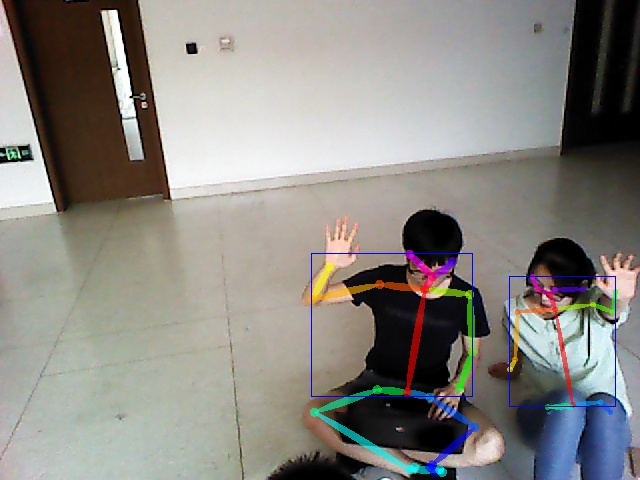
\includegraphics[width=0.8\textwidth]{wj.jpg}
    \caption{Waving judgement}
    \label{img_2}
  \end{figure}

  \begin{figure}
    \centering
    \subfigure[Input]{
      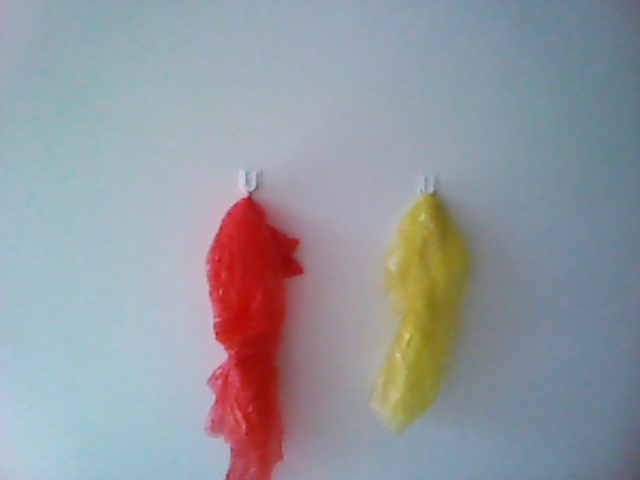
\includegraphics[width=0.4\textwidth]{input.jpg}
    }
    \subfigure[Salience map]{
      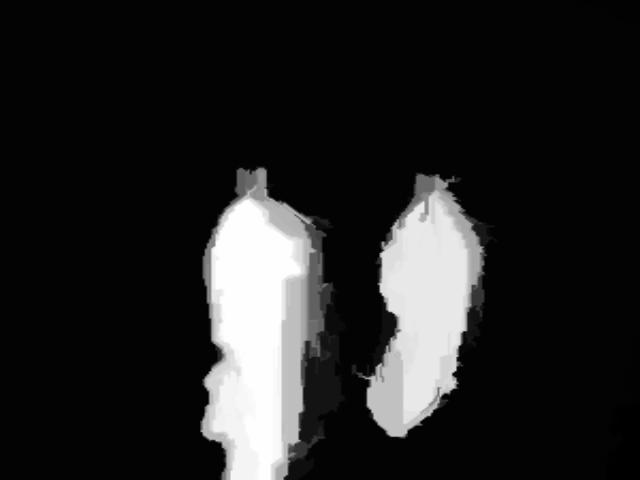
\includegraphics[width=0.4\textwidth]{salience.jpg}
    }
    \subfigure[Binary map]{
      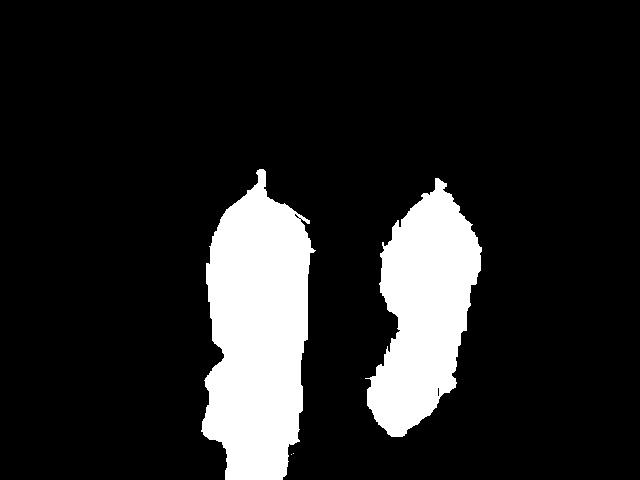
\includegraphics[width=0.4\textwidth]{binary.jpg}
    }
    \subfigure[Object detection]{
      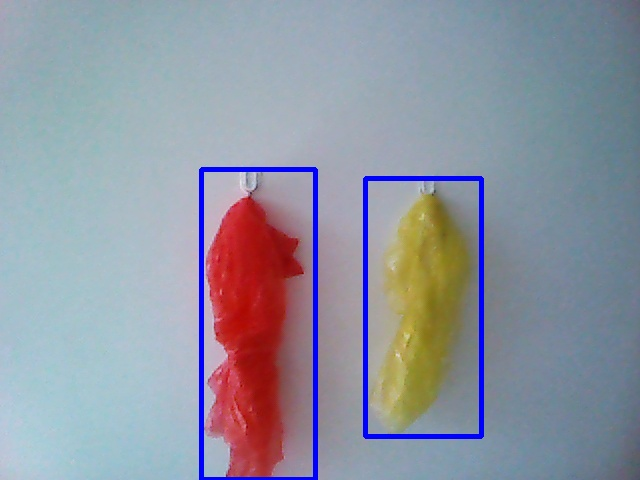
\includegraphics[width=0.4\textwidth]{detection.jpg}
    }
    \caption{Salience object detection}
    \label{img_3}
  \end{figure}


\section{Conclusion}
    I really love this experiment, thought there is still a lot of room for improvement, we solved some of tricky mission in farewell, like interaction. I'm familiar with ros, able to handle common problems. Also, I learned to cooperate with my partners. We made full use our strengths to complete tasks together. It's indeed a precious experience. Thanks my partners and Mr.Jeffrey for their help.

\begin{thebibliography}{99}
  \bibitem{openpose} Zhe Cao and Gines Hidalgo and Tomas Simon and Shih-En Wei and Yaser Sheikh. OpenPose: realtime multi-person 2D pose estimation using Part Affinity Fields[C]. 2018 IEEE Conference on Computer Vision and Pattern Recognition (CVPR). IEEE Computer Society, 2018.
  \bibitem{drfi} Huaizu Jiang, Jingdong Wang, Zejian Yuan, Yang Wu, Nanning Zheng, Shipeng Li. JSalient Object Detection: A Discriminative Regional Feature Integration Approach[C]. 2013 IEEE Conference on Computer Vision and Pattern Recognition (CVPR). IEEE Computer Society, 2013.
\end{document}
